
Este caso de prueba analiza el tópico noticioso referente del aborto, temática contingente que tomó la agenda nacional luego del anuncio presidencial del gobierno de Bachelet respecto a la reforma para su legalización.

El tópico comprende el periodo entre 1 de junio del 2014 y el 18 de febrero de 2015. Que comprende desde la primera etapa del anuncio del proyecto de ley de despenalización del aborto hasta el inicio de análisis de este tópico. 

Durante este proceso ocurrieron los siguientes hitos noticiosos contenidos en los tweets en todos los medios de prensa modelo (explicados en ~\ref{subsec:refnoticias}):

\begin{table}[H]
	\centering
	\begin{tabular}{| c | p{10cm} |}
		\hline
		Fecha    & Hito \\ \hline
		2 de junio 2014 & Comisiones de salud de las cámaras de diputados y senadores inician debate sobre proyectos de despenalización de aborto \\ \hline
		26 de junio 2014 & Anuncio del proyecto de despenalización del aborto \\ \hline
		24 de julio 2014 & ONU pide a Chile incluir violación como causa para hacerlo de forma legal \\ \hline
		3 de noviembre 2014 & Caso de joven de 13 años violada y embarazada \\ \hline
		30 de diciembre 2014 & Declaraciones de ministra de salud Henia Molina en la Segunda sobre los abortos en \emph{clínicas cuicas}\\ \hline
		30 de diciembre 2014 & Renuncia de ministra Henia Molina \\ \hline
		17 de enero 2015 & DC afirma que sus votos no estan asegurados para apoyar la despenalización del aborto \\ \hline
		1 de febrero 2015 & Declaraciones Rector PUC respecto a trabajadores que quieran realizar abortos en la Red UC \\ \hline
		5 de febrero 2015 & Red de clínicas privadas declara que no realizará abortos en sus recintos \\ \hline
		6 de febrero 2015 & Críticas a dichos de Lorenzini sobre los motivos, que a su juicio, causarían una violación \\ \hline
		9 de febrero 2015 & Cadem: 71\% aprueba proyecto de aborto enviado por el gobierno \\ \hline
	\end{tabular}
	\caption {Hitos noticiosos presentes en todos los medios de prensa modelos}
	\label{table:123_hitos_noticiosos}
\end{table}

\subsubsection{Procesamiento del tópico}

Durante el proceso de entrenamiento del clasificador se consideraron los siguientes criterios para realizar la selección:

\begin{itemize}
	\item Utilización del verbo abortar en un contexto no relacionado al tratamiento médico en cuestión.
	\item Insultos y agresiones 
	\item Comentarios demasiados generales que no permiten relacionar con el concepto aborto en cuestión.
\end{itemize}

Las cantidades según clasificación manual realizados en el proceso son los siguientes:

\begin{table}[H]
	\centering
	\begin{tabular}{| l | c | c | c |}
		\hline
		Clasificación    & Aceptados & Descartados & Total \\ \hline
		Entrenamiento    & 181 & 19 & 200\\ \hline
		Validación		 & 93 & 6 & 99\\ \hline
	\end{tabular}
	\caption {Clasificación referencia hecho noticioso}
\end{table}

Con esta información el clasificador del total de 1382 tweets aceptó 1357 tweets. \\

\subsubsection{Análisis de muestra representativa}

Para analizar el contenido de los tweets seleccionados se seleccionó una muestra representativa de los tweets que se refieren al título. La cual fue calculada considerando las siguientes variables:

\begin{itemize}
	\item Tamaño muestra $N = 1357$
	\item Error estándar $15\%$	
	\item Porcentaje estimado de la muestra $P = 0.9$
\end{itemize}

El tamaño de la muestra representativa de tweets para este tópico es de 309 tweets los cuales fueron seleccionados de manera aleatoria mediante el ordenamiento pseudoaleatorio entregado por la función \emph{RAND} de Mysql. \\

\subsubsection{Análisis de contenido}

Para realizar el análisis de contenido noticioso, se aplicó a la muestra de tweets el algoritmo explicado en \ref{fig:procedimientoTweetHN}. Con el cual se obtuvo la siguiente clasificación de los tweets de la muestra:

\begin{table}[h]
	\centering
	\begin{tabular}{| l | c | c |}
		\hline
		Clasificación    & Total & Porcentual\\ \hline
		Tweets que hacen referencia    & 108 & 34,95\%\\ \hline
		Tweets que no hacen referencia & 200 & 64,72\%\\ \hline
		    & 309 & 100\% \\
		\hline
	\end{tabular}
	\caption {Clasificación según referencia hecho noticioso}
\end{table}

\begin{table}[h]
	\centering
	\begin{tabular}{| l | c | c |}
		\hline
		Clasificación    & Total & Porcentual\\ \hline
		Opinión general (OG)  & 147 & 73,13\% \\ \hline
		Insumo Internacional (II) & 16 & 7,96\% \\ \hline
		Aporte a la discusión (AD) & 37 & 18,41\%\\ \hline
		No se refiere al tópico & 1 & 0,50\% \\ \hline
		& 201 & 100\% \\
		\hline
	\end{tabular}
	\caption {Clasificación de los tweets que no hacen referencia a un hecho noticioso}
	\label{clasifTweetsNoHechoNoticioso}
\end{table}

En la tabla \ref{clasifTweetsNoHechoNoticioso} se observa los efectivos resultados del filtro que determina si el tweet corresponde o no al tópico, donde sólo el 0,5\% de los tweets no están relacionados al tópico. La efectividad de este filtro  es fundamental para las etapas de clasificación
posteriores como la recolección de enlaces y análisis geográficos. 

El alto porcentaje de tweets del tópico que no se refieren a un hecho noticioso comprenden las distintas formas que frecuentan los usuarios para participar del debate público en Twitter: 73,3\% de estos tweets corresponden a una opinión personal, el 18,41\% entrega algún aporte a la discusión y el 7,96 \% corresponden a información o insumos internacionales.  

Estos resultados son alentadores en cuanto a la completitud y diversidad de esta información pues comprenden opiniones personales. enlaces externos, contexto internacional y referencias directas a hechos noticiosos. 

\begin{table}[H]
	\centering
	\begin{tabular}{| l | c | c | c | c | c | c |}
		\hline
		Clasificación    & \multicolumn{2}{c|}{La tercera} & \multicolumn{2}{c}{24 Horas} & \multicolumn{2}{|c|}{Bio-Bio} \\ \hline
		 
		Tweets con referencia a h.n.    & 49 & 15,86\% & 50 & 16,18\% & 45 & 14,56\% \\ \hline
		Tweets sin referencia a h.n. & 59 & 19,09\% & 58 & 18,77\% & 63 & 20,39\%  \\ \hline
		Total & 108 & 34,95\% & 108 & 34,95\% & 108 & 34,95\%  \\ \hline
	\end{tabular}
	\caption {Cobertura de hechos noticiosos (h.n.) contenidos en los tweets en los medios de prensa (Las cantidades porcentuales son respecto al total de la muestra)}
	\label{coberturaMediosModelo}
\end{table}

Al observar la tabla anterior \ref{coberturaMediosModelo} se observa que cerca del 50\% de los hechos noticiosos a los que se refieren los tweets no son cubiertos por alguno de los medios modelo, estos resultados expresan que es posible informarse de sucesos que no logran captar el interés del medio modelo para generar una nota de prensa logrando superar sus procesos de gatekeeping. De esto último podemos concluir que informarse de Twitter, permite informar de eventos que no son difundidos por los medios de prensa modelo.

El conjunto de tweets recogidos presenta 613 enlaces externos.

%\begin{table}[H]
%	\centering
%	\begin{tabular}{| l | c | c |}
%		\hline
%		Clasificación    & Total & Porcentual\\ \hline
%		Tweets que se refieren a un hecho noticioso difundido por el medio modelo  & 49 & 45,19\% \\ \hline
%		Tweets que se refieren a un hecho noticioso no difundido por el medio modelo & 56 & 53,85\% \\ \hline
%		& 104 & 100\% \\
%		\hline
%	\end{tabular}
%	\caption {Clasificación de los hechos noticiosos referenciados por los tweets, si son o no difundidos por el medio modelo de prensa convensional}
%\end{table}

\subsubsection{Análisis temporal}

\begin{figure}[H]
	\centering
	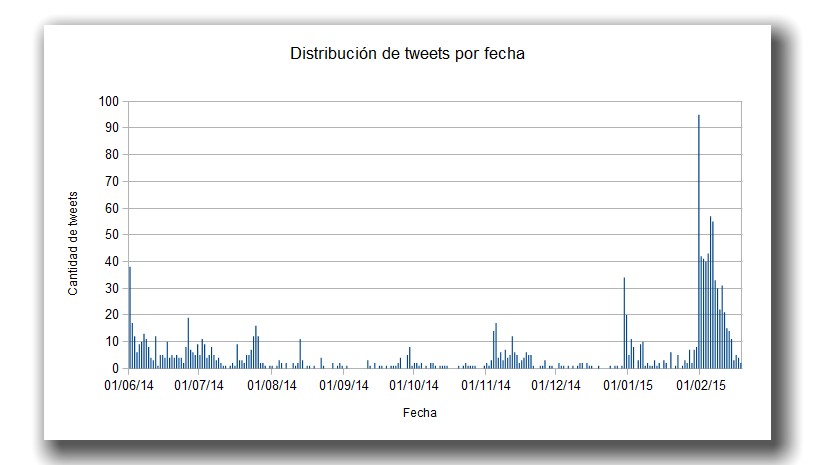
\includegraphics[width=1\textwidth]{imgs/123_general.png}
	\caption{Distribución de cantidad de tweets por día}
	\label{fig:123_tweets_por_dia}
\end{figure}

\begin{figure}[H]
	\centering
	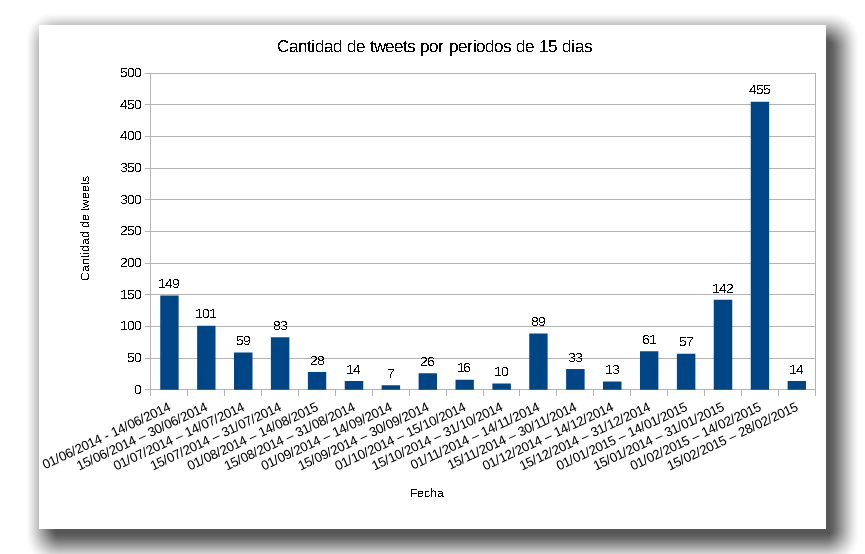
\includegraphics[width=1\textwidth]{imgs/cantidad_tweets_por_quincena_123_2.png}
	\caption{Distribución de cantidad de tweets por periodos de quince días}
	\label{fig:cantidad_tweets_por_quincena_123}
\end{figure}

En el gráfico \ref{fig:123_tweets_por_dia} es posible analizar la concentración de tweets por fecha, que en complemento del gráfico \ref{fig:cantidad_tweets_por_quincena_123} Nos permiten observar que existe una gran concentración de tweets en la primera quincena de febrero 2015 que se puede relacionar con la concentración de cuatros hitos noticiosos ocurridos desde el 1 de febrero hasta el 9 de febrero (ver tabla \ref{table:123_hitos_noticiosos}). El segundo periodo con más tweets corresponde a la primera quincena donde ocurrió un hito noticioso el 2 de junio de 2014. El tercer periodo con más tweets contiene un hito noticioso.(y dos hitos cercanos del periodo anterior, puesto que ocurrieron dos días antes del día previo del término del periodo). 

Es posible observar entonces que el debate se activa (y aumenta la cantidad de producción de tweets relacionados) en la medida que ocurren hechos noticiosos relevantes a nivel nacional.

\subsubsection{Análisis de re-tweet}

\begin{figure}[H]
	\centering
	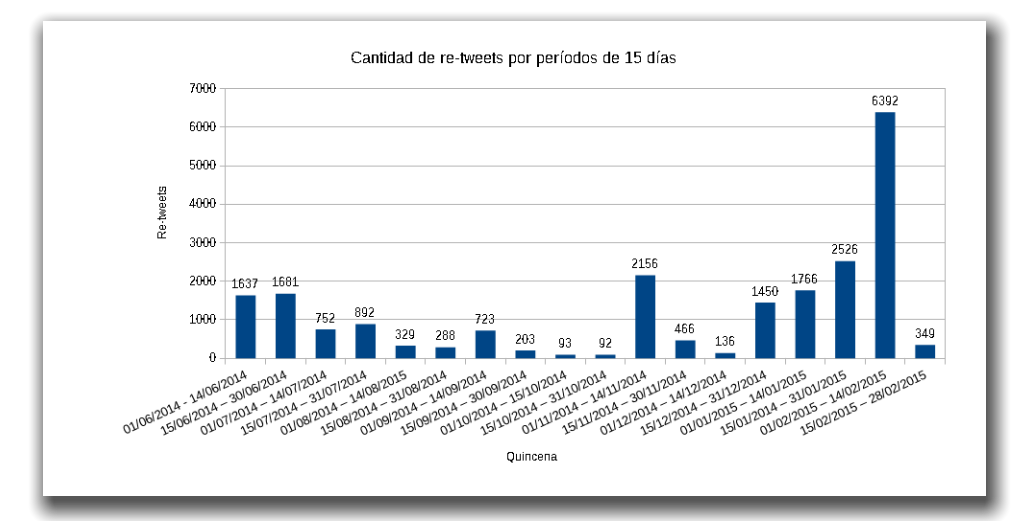
\includegraphics[width=1\textwidth]{imgs/123_cantidad_rt_por_quincena.png}
	\caption{Cantidad de re-tweets por quincena}
	\label{fig:123_cantidad_por_fecha}
\end{figure}

En el gráfico \ref{fig:123_tweets_por_dia} es posible analizar la concentración de tweets por periodo de tiempo, separados por quincena, el periodo de mayor concentración de tweets ocurre en la quincena 17 de manera similar a la mayor concentración de tweets analizados anteriormente, la segunda concentración ocurre en la segunda quincena de enero 2015  donde ocurre un hito noticioso, mientras que la tercera mayor concentración se ubica en la primera quincena del mes de noviembre 2014, donde se ubica un hito noticioso.

Según el razonamiento desarrollado para el \emph{ranking} de relevancia en ~\ref{subsubsec:orden-rel}. Los tweets con más RT son los que presentan información útil o relevante para quienes leyeron esos mensajes y realizaron la acción de re-tweet.

\begin{table}[H]
	\centering
	\begin{tabular}{| l | c | p{10cm} |}
		\hline
		Nº RT    & Autor & Texto de contenido\\ \hline
		1086  & @bairdCampbell & RT @fromerod: Los que prohibían el aborto,abortaban en  Londres.Hoy,quienes prohíben la libertad de expresión,se expresan en París. \\ \hline
		664  & @RosarioAlcaldeG & RT @joseantoniokast: Senador Lagos Weber tildo d "rasca" volante d la UDI sobre el aborto. Viendo esta foto sólo decir: Mira quien habla !  \\ \hline
		629  & @MAURYZS & RT @biobio: ONU recomienda a Chile permitir aborto a menores de 18 años por “salud fisiológica y mental” \\ \hline
		588  & @Beriiitha & RT @jmfmoran: Es menor, fue violada, quedó embarazada, no puede pagar un aborto, es obligada a parir un feto inviable. ¿Cuántas formas de v... \\ \hline
		360  & @raul\_torres79 & RT @link\_anarquista: Chile:Niña de 13 años embarazada por violación es castigada por el Estado sin derecho a aborto \\ \hline
		332  & @csuarezespinoza & RT @DerechaTuitera: Levantemos la mano todos los que creemos que el aborto provoca daños sicológicos irreparables! (acá un ejemplo) http \\ \hline
		253  & @RuubiaNaturaal & RT @lasultimas: Van Rysselberghe:"El aborto terapéutico es un control de calidad a la raza humana". Envía "weona loca" al 6969 y recibe chi \\ \hline
		252  & @urpiestrada & RT @PorAbortoLegal: Quién decide sobre un \#Aborto? explicación sencilla  http://t.co/cP4ApMZw33 \#provida \\ \hline
		243  & @irutherf & RT @KennethOficial: ¡Que ironía! Los que están a favor del aborto... nacieron. \\ \hline
		242  & @zarasenda & RT @SomosDocumental: Cine militante y documental contra la reforma de la Ley del aborto. http://t.co/NDfoNF4ABM \#TrendelaLibertad \\ \hline
	\end{tabular}
	\caption {10 Tweets mas re-twiteados del tópico}
	\label{table:123_topten_rt}
\end{table}

Si analizamos los tweets en \ref{table:123_topten_rt} es posible observar que 7 de los 10 cuentan con una imagen adjunta al tweet. De éstos 4 se refieren a un hecho noticioso, 4 se refieren a opiniones personales, 1 aporte a la discusión y 1 correspondiente a información internacional sobre el tema. 

\begin{table}[H]
	\centering
	\begin{tabular}{| c | c |}
		\hline
		\multicolumn{1}{|p{3cm}|}{Número de tweets emitidos por un mismo usuario} & \multicolumn{1}{p{3cm}|}{Número de usuarios  distintos} \\ \hline
		1 & 602 \\ \hline
		2 & 130 \\ \hline
		3 & 41  \\ \hline
		4 & 27 \\ \hline
		5 & 4  \\ \hline
		6 & 9  \\ \hline
		7 & 4  \\ \hline
		8 & 3  \\ \hline
		9 & 1  \\ \hline
		10 & 2  \\ \hline
		11 & 3  \\ \hline
		12 & 1  \\ \hline
		15 & 1  \\ \hline
		16 & 2  \\ \hline
		17 & 1  \\ \hline
	\end{tabular}
	\caption {Cantidad de usuarios distintos por número de tweets emitidos}
\end{table}

\subsubsection{Análisis geográfico}

La distribución de usuarios que realizaron tweets en el tópicos, con una ubicación 
identificada fueron 223 de los 831 autores distintos (26,8\%).

\begin{figure}[H]
	\centering
	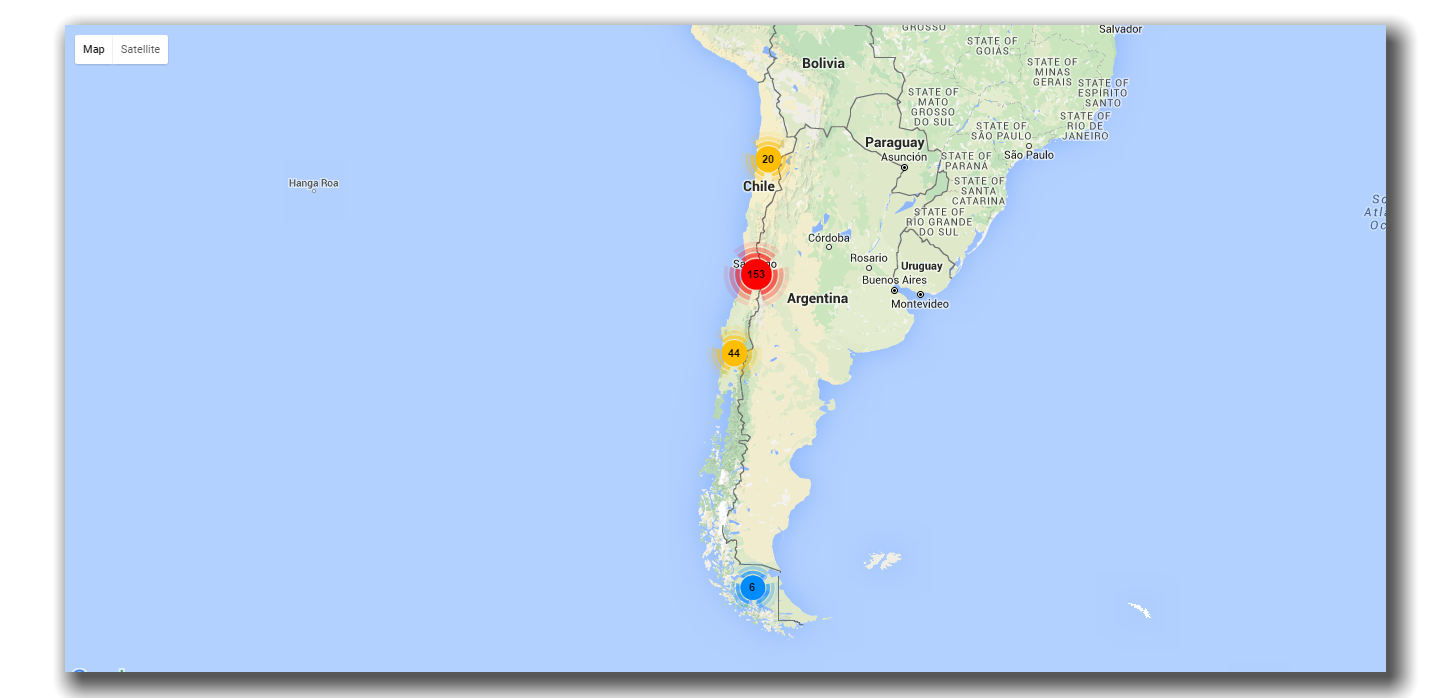
\includegraphics[width=1\textwidth]{imgs/213_usuarios_mapa.png}
	\caption{Distribución geográfica de los usuarios}
	\label{fig:geo_usuarios_213}
\end{figure}

